\documentclass[twoside]{article}

\usepackage{lipsum}
\usepackage[none]{hyphenat} 

\usepackage[sc]{mathpazo} 
\usepackage[T1]{fontenc} 
\linespread{1.05}
\usepackage{microtype}

\usepackage[hmarginratio=1:1,top=32mm,columnsep=20pt]{geometry}
\usepackage{multicol} 
\usepackage[hang, small,labelfont=bf,up,textfont=it,up]{caption} 
\usepackage{booktabs} 
\usepackage{float} 
\usepackage{hyperref}
\usepackage{amsmath}

\usepackage{lettrine} 
\usepackage{paralist}

\usepackage{abstract} 
\renewcommand{\abstractnamefont}{\normalfont\bfseries}
\renewcommand{\abstracttextfont}{\normalfont\small\itshape} 

\usepackage{titlesec} 
\renewcommand\thesection{\Roman{section}} 
\renewcommand\thesubsection{\Roman{subsection}} 
\titleformat{\section}[block]{\large\scshape\centering}{\thesection.}{1em}{} 
\titleformat{\subsection}[block]{\large}{\thesubsection.}{1em}{}

\usepackage{fancyhdr} 
\pagestyle{fancy} 
\fancyhead{} 
\fancyfoot{}

\fancyhead[C]{ Estad\'istica $\bullet$ Equipo 5 $\bullet$ C-411}
\fancyfoot[RO,LE]{\thepage}

\title{\vspace{-0.5cm}\fontsize{20pt}{10pt}\selectfont\textbf{Proyecto Fase 2}}

\author{
\large
\textsc{\vspace{-2cm} Alejandro Campos, Darian Dominguez, Nelson Mendoza}\\[3.5cm]
\normalsize Facultad de Matem\'atica y Computaci\'on \\
\normalsize Universidad de la Habana \\
\normalsize 2021 \\
\vspace{-5mm}
}
\date{}


\usepackage{graphicx}
\begin{document}

\maketitle

\thispagestyle{fancy} 

\begin{center}
\textbf{Resumen}
\end{center}
\noindent \textit{Resumen here}\\

\begin{multicols}{2}

\section{Introduci\'on}
introduction here





\section{Set de datos}
El set de datos que se analizar\'a a continuaci\'on es el conjunto de datos de Delft, utilizado para predecir el rendimiento hidrodin\'amico de los yates de vela a partir de las dimensiones y velocidad. Esta base de datos muestra el comportamiento de las siguientes variables:
\begin{enumerate}
\item Posici\'on longitudinal del centro de flotabilidad, adimensional.
\item Coeficiente prism\'atico, adimensional.
\item Relaci\'on longitud-desplazamiento, adimensional.
\item Relaci\'on haz-tiro, adimensional.
\item Relaci\'on longitud-haz, adimensional.
\item N\'umero de Froude, adimensional.
\item Resistencia residual por unidad de peso de desplazamiento, adimensional.\\
\end{enumerate}

\subsection{Variables principales}
De las variables anteriores se catalogan como principales, por su importancia, el coeficiente prism\'atico, el n\'umero de Froude y la resistencia residual. El coeficiente prism\'atico nos da una idea de c\'omo est\'a dise\~nado el barco para "penetrar" en el agua, es decir, la facilidad para que el barco se ponga a planear y aumente su velocidad. Indica, adem\'as, la relaci\'on entre el volumen sumergido y el volumen definido por su manga m\'axima. Dicho de otra manera, indica el cociente entre el volumen sumergido y el volumen de la pieza a partir de la cual se ha podido "tallar" el casco. Cuanto menor sea este coeficiente m\'as finos ser\'an la popa y proa y, por tanto, mejor afrontar\'an las olas. El n\'umero de Froude relaciona el efecto de las fuerzas de inercia y las fuerzas de gravedad que act\'uan sobre un fluido, estas fuerzas est\'an presentes en el accionar de las olas causadas por un barco al navegar, por ello, esta variable es de suma importancia para el rendimiento hidrodin\'amico de un buque. Con el n\'umero de Froude se puede predecir la resistencia al avance de los barcos, estimando la resistencia que estos presentan ante las olas, que depende de la resistencia de fricci\'on (debida a la superficie mojada del casco) y la resistencia residual (debida a la formaci\'on de olas). Finalmente, la resistencia residual por unidad de peso de desplazamiento es causada por la presi\'on que genera el casco al abrirse paso a trav\'es del agua, esta variable es de gran valor para los yates de vela en la etapa de dise\~no inicial,  para evaluar el rendimiento del buque y estimar la potencia propulsora requerida.\\





\section{Regresi\'on lineal}
Utilizaremos el m\'etodo backward para realizar un modelo de regresi\'on lineal que explique el comportamiento de la resistencia residual. Luego nuestro modelo comienza con todas las variables principales, analicemos los resultados:\\

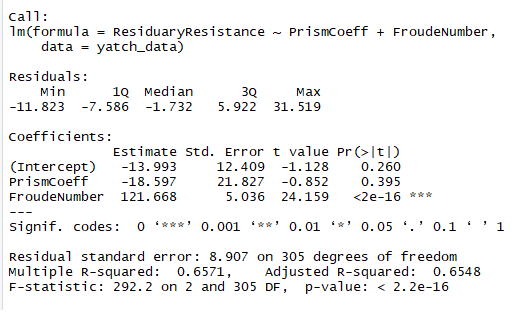
\includegraphics[scale = 0.5]{images/pic_01.png} \\

Podemos observar que la variable coeficiente prism\'atico (\textit{PrismCoeff}) ni el intercepto son significativos en el modelo, es decir, sus coeficientes no le aportan nada a este. \\
Si analizamos la matriz de correlaci\'on obtenemos: \\

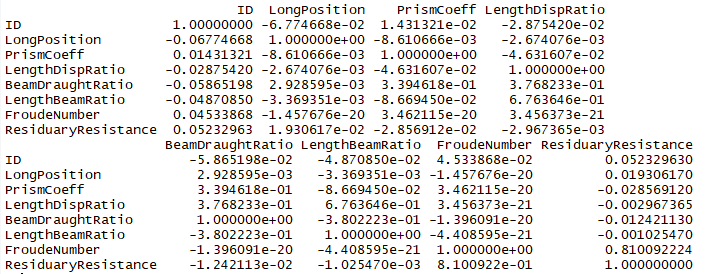
\includegraphics[scale = 0.4]{images/pic_02.png} \\

Al analizar la matriz es f\'acil darse cuenta de que las variables coeficiente prism\'atico y resistencia residual no est\'an correlacionadas, de hecho, ninguna de las variables est\'an correlacionadas entre s\'i, a excepci\'on del n\'umero de Froude y resistenia residual. Como en el caso de este modelo en particular la variable dependiente \textit{ResiduaryResistance} no est\'a correlacionada con la variable independente \textit{PrismCoeff}, debemos eliminarla. Por lo tanto tenemos un nuevo modelo sin la variable \textit{PrismCoeff} que, adem\'as hab\'iamos visto, no era significativa.\\

Luego llegamos a un modelo que tiene a \textit{ResiduaryResistance} como variable dependiente y a \textit{FroudeNumber} como variable independiente. Los resultados obtenidos con este modelo son los siguientes:\\

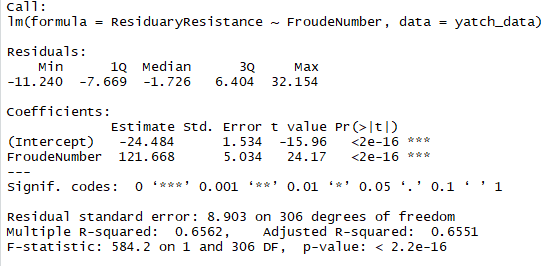
\includegraphics[scale = 0.4]{images/pic_03.png} \\

Ahora tenemos que Pr($>|t|$) de la variable independiente y del intercepto son menores que $0.05$. El p-value tambi\'en es menor que $0.05$. Por lo tanto, podemos proceder a hacer un an\'alisis de la presici\'on del modelo.\\
El modelo resultante es:
$$\hat{ResiduaryResistance} = -24.484 + 121.668 * FroudeNumber$$

Se observa que el coeficiente del intercepto es mucho menor que el coeficiente del n\'umero de Froude, por lo tanto podemos decir que la mayor parte de la resistencia residual de los barcos est\'a explicada a partir del n\'umero de Froude. El coeficiente del n\'umero de Froude es significativo al $0\%$ y el del intercepto tambi\'en es significativo al $0\%$. Analizando los valores de estos coeficientes, se puede afirmar que por cada aumento unitario en el n\'umero de Froude debemos esperar que la resistencia residual aumente en $121.668$. \\

Pasando al an\'alisis de los residuos tenemos que el R-cuadrado ajustado es $0.66$, menor que $0.70$ por lo que podemos decir que  es un modelo bastante malo, no obstante, sigamos con el an\'alisis. El error est\'andar es $8.9$, no es tan peque\~no, no es lo ideal. El p-value del estad\'igrafo F, como se hab\'ia dicho, es menor que $0.05$, lo que quiere decir que existe al menos una variable significativamente diferente a cero en el modelo.\\

Veamos ahora si el modelo cumple los supuestos.\\
Recordemos que los supuestos son:
\begin{enumerate}
\item Existe una relaci\'on lineal entre las variables dependientes e independientes.
\item Los errores ($e_1,...,e_n$) son independientes.
\item El valor esperado del error aleatorio $e_i$ es cero ($E(e_i) = 0$)
\item La Varianza del error aleatorio es constante ($V(e_i) = \theta^2$). Homocedasticidad.
\item Los errores adem\'as de ser independientes son id\'enticamente distribuidos y siguen distribución normal con media cero y varianza constante ($e_i ~ N(0, \theta^2)$)
\item Las variables independientes del modelo no est\'an correlacionadas.
\end{enumerate}

Los supuestos $1$ y $6$ se cumplen en el modelo en cuesti\'on, pues el n\'umero de Froude esta correlacionado con la resistencia residual (ver matriz de correlaci\'on) y no hay m\'as variables independientes que el mismo n\'umero de Froude.\\
Realicemos un an\'alisis de los residuos para verificar si el resto de los supuestos se cumple:\\

Para analizar el cumplimiento del supuesto $3$ debemos verificar si la media de los errores es cero y la suma de los errores es cero. Con ayuda de los comandos de R, \textbf{mean} y \textbf{sum}, se llega a que, en efecto, este supuesto se cumple.\\

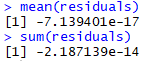
\includegraphics[scale = 0.7]{images/pic_04.png} \\

Para verificar el cumplimiento del supuesto $5$ debemos comprobar si los errores est\'an normalmente distribuidos. El histograma de residuos y el gr\'afico QQ-plot son formas de evaluar visualmente si los residuos siguen una distribuci\'on normal. Por tanto, buscamos que el histograma tenga forma de campana y en el QQ-plot que la mayor\'ia de los puntos de los residuos se encuentren sobre la recta o muy cercana a ella. Con ayuda de R construimos los gr\'aficos antes mencionados para este modelo:\\

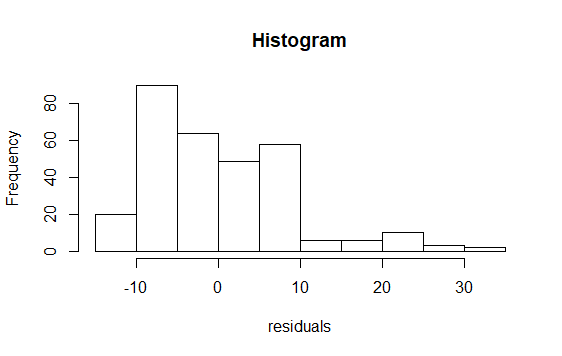
\includegraphics[scale = 0.4]{images/pic_05.png} \\
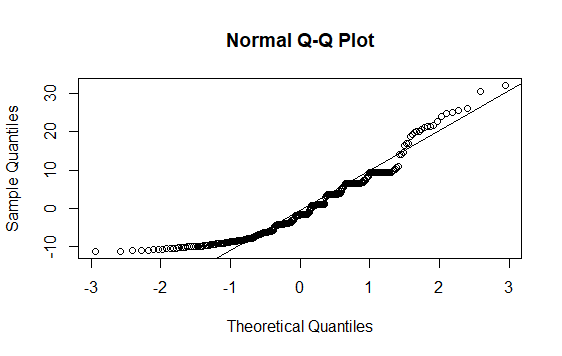
\includegraphics[scale=0.4]{images/pic_06.png} \\

Parece que los residuos no siguen una distribuci\'on normal, comprob\'emoslo con el test de Shapiro-Wilk, con ayuda de R.\\

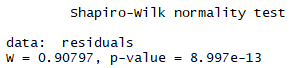
\includegraphics[scale = 0.6]{images/pic_07.png} \\

Como se observa, el p-valor del test de Shapiro-wilk es menor que $0.05$, luego se rechaza la hip\'otesis nula por lo que los errores no siguen una distribuci\'on normal. Ya hab\'iamos visto que este modelo era bastante malo, y ahora no cumple uno de los supuestos, por lo tanto ya podemos desecharlo. Sin embargo, analicemos el resto de los supuestos.\\

La prueba Durbin-Watson se usa para probar si los residuos son independientes. La hip\'otesis nula de esta prueba es que los errores son independientes.\\

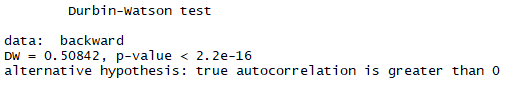
\includegraphics[scale=0.5]{images/pic_08.png} \\

Como el p-valor de esta prueba es menor que $0.05$ se rechaza la hip\'otesis nula, por lo que podemos afirmar que tampoco se cumple el supuesto $2$.\\

Para probar el supuesto $4$ de la Homocedasticidad podemos graficar los residuos como se muestra a continuaci\'on:\\

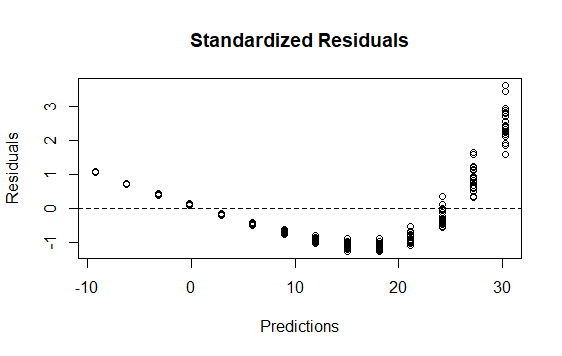
\includegraphics[scale = 0.4]{images/pic_09.png} \\
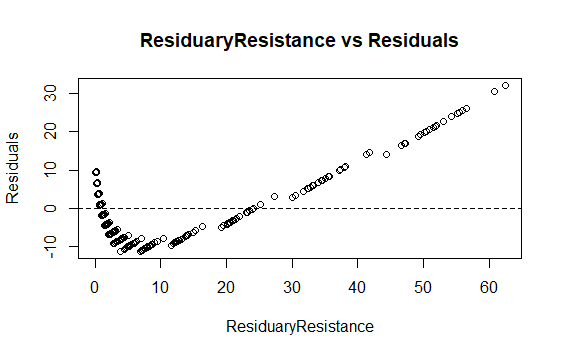
\includegraphics[scale=0.4]{images/pic_10.png} \\

Con estos gr\'aficos se comprueba que estos puntos no siguen una franja, por lo que es muy probable que este supuesto tampoco se cumpla. Utilicemos la prueba de Breusch-Pagan, que se utiliza para determinar la heterocedasticidad en un modelo de regresi\'on lineal, para verificar lo anterior.\\

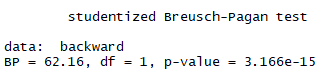
\includegraphics[scale=0.6]{images/pic_11.png} \\

Como el p-valor de esta prueba es menor que $0.05$ se rechaza la hip\'otesis nula por lo que  podemos afirmar que se cumple la heterocedasticidad. Por lo que el supuesto de Homocedasticidad no se cumple.\\\\

Se concluye que para estos datos no existe un modelo de regresi\'on lineal que se ajuste a ellos. 

No podemos dejar de mencionar que, dado el an\'alisis de la matriz de correlaci\'on realizado en esta secci\'on, no es posible utilizar otra combinaci\'on de variables para realizar otro modelo de regresi\'on, ya que las variables no tienen correlaci\'on entre s\'i, a excepci\'on de las que se analizaron. El \'unico modelo que se podr\'ia hacer con estos datos fue el que analizamos anteriormente, ya que el resto de combinaciones de modelos posibles no cumple, a priori, el supuesto $1$.

El an\'alisis de correlaci\'on tambi\'en se aborda de una forma mejor explicativa en la secci\'on X del presente informe.\\\\



\section{ANOVA}
Realicemos un an\'alisis de ANOVA a fin de investigar si el n\'umero de Froude afecta la resistencia residual de los barcos veleros. Adem\'as, debemos considerar como factor secundario el coeficiente prism\'atico de estos. Es decir, tenemos la variable de estudio \textit{ResiduaryResistance}, y es claro que el n\'umero de Froude se puede ver como tratamiento y el coeficiente prism\'atico como bloque.

Luego el problema que acabamos de plantear responde al siguiente modelo estad\'istico de bloques: 
$$Y_{ij} = \mu + \alpha_i + \beta_j + e_{ij}$$ 
Donde $Y_{ij}$ es la medici\'on que corresponde al tratamiento $i$ y al bloque $j$, en este caso la resistencia residual de los barcos; $\mu$ es la media global poblacional; $\alpha_i$ es el efecto debido al tratamiento $i$, en este caso los distintos n\'umeros de Froude; $\beta_j$ es el efecto debido al bloque $j$, en este caso los distintos coeficientes prism\'aticos, y $e_{ij}$ es el error aleatorio atribuible a la medici\'on $Y_{ij}$.\\

La hip\'otesis que debemos formular es la siguiente:
\begin{align*}
H_0 &: \mu_1 = \mu_2 = ... = \mu_{14} = \mu \\
H_1 &: \mu_i \neq \mu_j \hspace{0.3cm} \text{para alg\'un} \hspace{0.3cm} i \neq j
\end{align*}

La cual se puede reescribir de forma equivalente como:
\begin{align*}
H_0 &: \alpha_1 = \alpha_2 = ... = \alpha_{14} = 0 \\
H_1 &: \alpha_i \neq 0 \hspace{0.3cm} \text{para alg\'un} \hspace{0.3cm} i 
\end{align*}

Primero deber\'iamos acomodar los datos para poder trabajar con ellos. Lo que buscamos es tenerlos de la siguiente forma:\\

\resizebox{6.5cm}{!}{
\begin{tabular}{| c | c | c |}
\hline
FroudeNumber & PrismCoeff & ResiduaryRes \\ \hline
f1 & p1 & r1 \\
f1 & p2 & r2 \\
f1 & p3 & r3 \\
\vdots & \vdots & \vdots \\
f1 & p10 & r10 \\
f2 & p1 & r11 \\
\vdots & \vdots & \vdots \\
f14 & p10 & r308 \\ \hline
\end{tabular}} \\\\

Como tenemos $14$ n\'umeros de Froude distintos y $10$ coeficientes prism\'aticos distintos, entonces ponemos en la primera columna secuencialmente $10$ veces el primer n\'umero de Froude, luego el segundo y as\'i sucesivamente, para poder listar en la segunda columna los valores de los coeficientes prism\'aticos en cada caso y, por \'ultimo, listar la resistencia residual de cada barco.\\

Luego necesitamos comparar las medias de los $14$ niveles del factor y las medias de los $10$ niveles del bloque. Para esto realizamos gr\'aficos de cajas con las medias de cada uno.\\

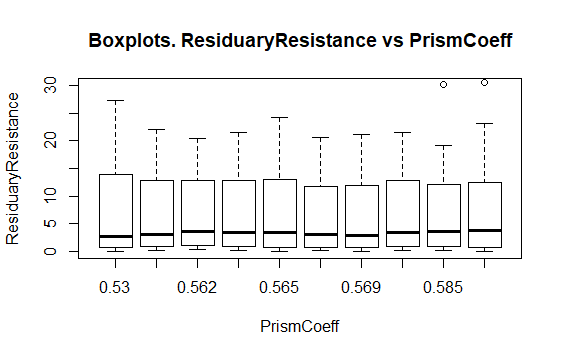
\includegraphics[scale = 0.4]{images/pic_12.png} \\
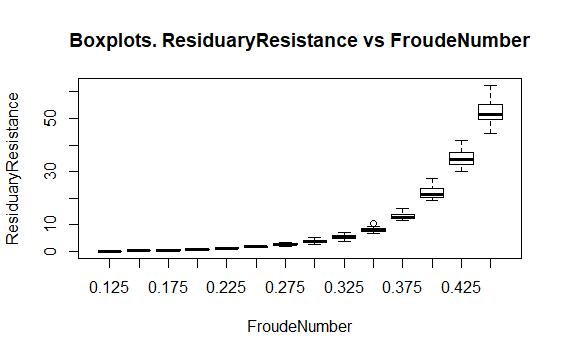
\includegraphics[scale=0.4]{images/pic_13.png} \\

Podemos observar que las medias de la resistencia residual de los coeficientes prism\'aticos son bastante cercanas, oscilando entre $2$ y $3$ aproximadamente, por lo que es posible que el coeficiente prism\'atico no tenga efecto sobre la resistencia residual de los veleros. 

Por otro lado, el gr\'afico de la resistencia residual y el n\'umero de Froude muestra mucha diferencia en las medias, podemos apreciar que empieza en valores muy cercanos a $0$ y, a medida que el n\'umero de Froude aumenta, obtenemos valores de resistencia residual promedio de $50$. Por lo tanto, es muy probable que el n\'umero de Froude tenga efecto sobre la resistencia residual de los veleros.\\

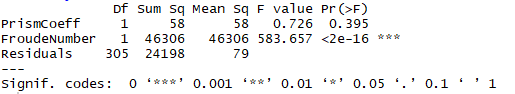
\includegraphics[scale = 0.4]{images/pic_14.png} \\

Notamos que en el caso del coeficiente prism\'atico el p-valor es mayor que $0.05$, luego no podemos rechazar $H_0$ por lo que se acepta que este no influye en la resistencia residual de los barcos.

En el caso del n\'umero de Froude, como el p-valor es menor que la significaci\'on prefijada $\alpha = 0.05$, entonces se rechaza $H_0$ y se acepta que al menos un par de n\'umeros de Froude tienen una resistencia promedio diferente, es decir, influyen sobre la resistencia residual de los barcos.\\

Verifiquemos si el modelo cumple los supuestos. Recordemos que estos son:
\begin{enumerate}
\item Los $e_{ij}$ siguen una distribuci\'on normal con media cero. 
\item Los $e_{ij}$ son independientes entre s\'i. 
\item Los residuos de cada tratamiento tienen la misma varianza $\theta^2$.\\
\end{enumerate}

Para verificar el cumplimiento del supuesto $1$ debemos comprobar si los errores est\'an normalmente distribuidos. El histograma de residuos y el gr\'afico QQ-plot son formas de evaluar visualmente si los residuos siguen una distribuci\'on normal. Por tanto, buscamos que el histograma tenga forma de campana y en el QQ-plot que la mayor\'ia de los puntos de los residuos se encuentren sobre la recta o muy cercana a ella. Con ayuda de R construimos los gr\'aficos antes mencionados para este modelo:\\

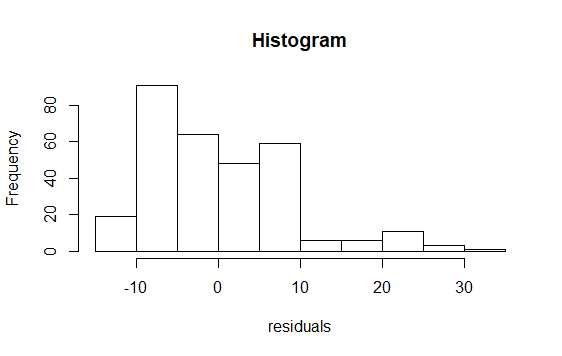
\includegraphics[scale = 0.4]{images/pic_15.png}
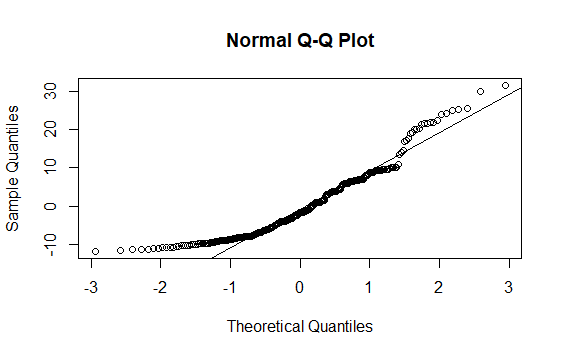
\includegraphics[scale=0.4]{images/pic_16.png} \\

Parece que los residuos no siguen una distribuci\'on normal, utilizaremos el test de Shapiro-Wilk, con ayuda de R, para comprobarlo.\\

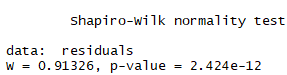
\includegraphics[scale = 0.6]{images/pic_17.png} \\

Como se observa, el p-valor del test de Shapiro-wilk es menor que $0.05$, luego se rechaza la hip\'otesis nula por lo que los errores no siguen una distribuci\'on normal. Podemos desechar este modelo, no obstante, analicemos el resto de los supuestos.\\

La prueba Durbin-Watson se usa para probar si los residuos son independientes. La hip\'otesis nula de esta prueba es que los errores son independientes.\\

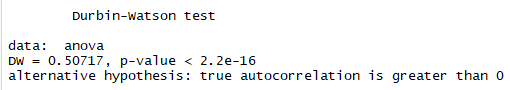
\includegraphics[scale = 0.5]{images/pic_18.png} \\

Como el p-valor de esta prueba es menor que $0.05$ se rechaza la hip\'otesis nula, por lo que podemos afirmar que tampoco se cumple el supuesto $2$.\\

Por \'ultimo, para probar el supuesto $3$ de la Homocedasticidad podemos graficar los residuos como se muestra a continuaci\'on:\\

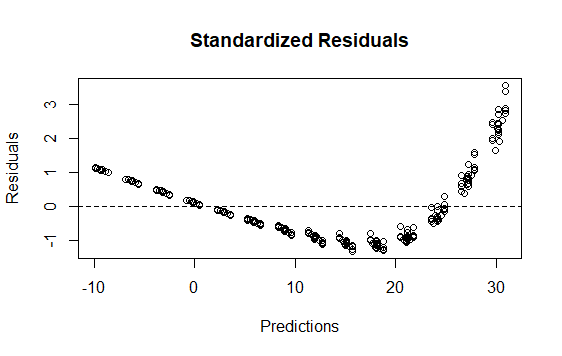
\includegraphics[scale = 0.4]{images/pic_19.png} \\

Los puntos no forman una franja, parece ser no que tienen varianza constante. Utilicemos la prueba de Bartlett para confirmarlo.\\

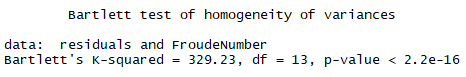
\includegraphics[scale = 0.5]{images/pic_20.png} \\

Como el p-valor de esta prueba es menor que $0.05$ se rechaza la hip\'otesis nula por lo que el supuesto de Homocedasticidad no se cumple.\\\\

De forma an\'aloga a como se desarroll\'o en esta secci\'on, se realizaron varios an\'alisis de ANOVA considerando otras variables, pero por desgracia ninguno result\'o v\'alido. Solo se refleja en este informe el realizado con las variables principales visto anterioremente.\\\\



\section{Reducci\'on de dimensi\'on}

\end{multicols}{2}
\end{document}